\chapter{Open Microfluidics}\footnote{This chapter has been modified from the manuscript in preparation of the same title. The manuscript includes as authors Erwin Berthier, Theodorus de Groot, Jean Berthier, Benjamin Casavant, and David Beebe}
\label{Chap:OpenMicrofluidics}


Microfluidics has demonstrated fundamentally unique capabilities in a broad range of areas such as medicine, diagnostics, cell biology, and analytical chemistry. However, challenges in manufacturing and difficulties in reliably using microfluidic systems limit their widespread adoption and translation. Despite the development of disruptive microfluidic paradigms such as soft-lithography, stereo-lithography additive (SLA) 3D-printing, and paper microfluidics, there remains an unmet need for a technology that enables cost-effective manufacturing while also providing a high degree of control over the fluid exchanges. Here, we present advances in open microfluidics that have the potential of being manufactured using standard manufacturing processes, provide control over fluid flows on par with traditional microfluidic systems, and enable unique modes of interaction and reconfigurability of the fluid paths.


\section{Introduction}
The last decade has seen a fundamental rise in the adoption and translation of microfluidic systems into diagnostic, clinical research, and analytical systems applications (e.g. point-of-care systems, mass-spectrometry, etc). The driving factors of this gain in popularity are the need for smaller sample volumes, particularly in the case of rare samples (such as pediatric blood, stem cells, etc) \cite{Burns1998, Ingham2007,Song2006a,Thorsen2002a}, the ability to quantify phenomena at a single molecule or cell level (as is used in digital PCR / ELISA or circulating tumor cell analysis) \cite{Hong2012,Kopp1998,Song2006a}, and engineering platforms of higher relevance to the system being studied \cite{Berthier2010, Domenech2009, Huh2010a,Jeon2015,Meyvantsson2008a,Moraes2013,Sackmann2014a}. Despite unique features, microfluidics inherently imposes usability and manufacturing challenges that limit adoption. Manufacturing enclosed microchannels remains a significant bottleneck of microfluidic fabrication, despite years of research and hundreds of papers published, that leads to high costs and reliability concerns \cite{Guckenberger2015,Sackmann2014,Shiu2008RapidEmbossing}. Further, the leading microfluidic manufacturers on the market today closely guard the processes they have developed to solve specific challenges, which increases the cost of fabrication and limits the ability to perform early stage prototyping. The difficulty of use by non-experts and poor reliability track-record is another major challenge of traditional microfluidic systems leading to high user error and maintenance cost in the case of fully integrated "black-box" systems \cite{Casavant2013,Sackmann2014}. Here, we present advances in open microfluidics, a novel approach to designing microfluidic systems that combines high-levels of fluidic control on par with traditional closed microfluidic systems while also enabling standard low-cost manufacturing processes, simplicity of use, and incomparable reliability of operation.

The development of simple methods that lower the barriers of adoption for microfluidic systems (fabrication complexity, ease-of-use) has been an intense focus of research and led to exponential growth in adoption and number of publications \cite{Berthier2012,Sackmann2014a}. The initial widely recognized development in microfabrication that unlocked the field for widespread adoption is soft lithography and the use of silicone polymers for device fabrication \cite{Xia1998a}. Other developments of importance to medicine and diagnostics that expanded the breadth of applications was the use of thermoplastics through micromilling \cite{Guckenberger2015b, Wilson2011}, hot-embossing \cite{Shiu2008RapidEmbossing, Young2011}, or laser cutting \cite{Klank2002, Yuen2010Low-costCutter}. The emergence of high-resolution stereolithography additive printing (SLA, a form of 3D-printing) is promising to rapidly transform the field of microfluidics as fully enclosed microdevices can be fabricated in hours from design-to-prototype \cite{Au20163D-PrintedMicrofluidics, Bhargava2014}. SLA imposes important material limitations (e.g. limited biocompatibility and proprietary resins) and remains an expensive solution more adapted to prototyping and custom “one-off” designs. The development of paper-microfluidics, in which fluid is guided by a printed paper matrix, is showing great promise to becoming the next generation ultra-low cost diagnostic systems \cite{Martinez2008, Osborn2010a,Park2013a}. Paper-based devices are incredibly cost-effective to produce, user-friendly and intuitive to operate, and reliable to use since they do not require pressure sources, seals, and cannot fail due to air bubbles. However, handling biological fluids in paper is limited, in particular the ability to exchange and wash fluids, and material interaction and adsorption challenges are increased due to the high surface-to-volume ratios. Despite very appealing advances in microfluidic technologies, there remains a tradeoff between control over the fluid and operational simplicity.

Open microfluidics describes the flow of fluids in channels that have one or more open faces; the simplest being a rectangular channel with no ceiling \cite{Berthier2012,Casavant2013}. Open microfluidics allows the control over fluids on-par with traditional closed-fluidics while providing manufacturing simplicity and reliability of use on par with paper-microfluidics. In open microfluidics, fluid flow is driven by capillary force provided by the solid parts of the cross section of the channel allowing the fluid to span over the open sections of the cross section. We compile and highlight here the initial forays of open microfluidics and expand on them to demonstrate the enabling potential to create microfluidic systems with unique reliability, access to the fluid flows, and ease of prototyping and manufacturing. We show that open microfluidics is a technology that enables control over fluid handling, access to the sample throughout the device operation, simple manufacturing and prototyping (compatible with injection molding and 3D printing), and the potential to create non-planar reconfigurable systems. Finally, we show that reconfigurable systems can be created utilizing the example of Lego-like blocks that enable the creation of a bread-board microfluidic system that can be modified during the operation of the device.

\section{Methods}
\subsection{Open microfluidic 3D printing}
Open microfluidic models were designed using the CAD software Solidworks 2016 (Dassault systems, source files available in the supplementary information) and exported into a STEP file format. STEP files were printed in accura 25 resin on a high-resolution Viper 2000 SLA printer from 3D systems (Midwest prototyping, Blue mounds, WI). The parts were printed using the orientation in which they were designed in the CAD software in high-resolution with a Z-compensation set to 0. After removed from the printer, the parts were washed in isopropyl-alcohol for 2 min while gently shaking them; the support features were removed and the parts washed again for 2 min; the parts were air dried and placed in a UV curing oven for 20 min to finalize the curing of the resin; the support features on the bottom side were gently sanded by hand.

\subection{Open microfluidic channel preparation}
The 3D printed parts were treated for hydrophilization using a Diener Zepto plasma treater (Ebhausen, Germany), using the following parameters: plasma pressure set at 5 KPa, O2 gas flush for 30 sec at constant pressure, plasma power set at 50\%, plasma treatment time of 1 min. Once removed from the plasma treater, the outer surfaces of the 3D printed parts were wiped with a kimwipe to induce hydrophobic recovery(D.J. Guckenberger, Berthier, Young, & Beebe, 2012). In the case of the digital microfluidic application presented in Figure 4B, the outer surface of the microwell part were wiped with hydrophobic carnauba wax to further improve the hydrophobic treatment. In brief, a kimwipe was gently rubbed against the wax and a thin layer of way was delivered on the top surface of the 3D printed part. 

\subsection{Open microfluidic flows}
The fluid used to visualize flows were prepared by using food colorant (McCormick, Sparks, MD) in water in a dilution of 250 uL colorant in 10 mL of water. Fluid was pipetted using a Gilson 20-200 uL manual pipettor. Images were captured using a Nikon D100 camera.

\section{Results and discussion}

\subsection{Open microfluidic conditions for flow}
Open microfluidics is a class of microfluidic channels that are defined as having one or more open-air interfaces along the path of the channels (Figure \ref{figure:Fig1}A). The open aspect of the microchannels rely on surface tension for fluid flow to occur, similarly to what is observed in paper-microfluidics. Open microfluidics flows are thus simple and reliable as they do not rely on external actuators, require liquid tight seals, and are not affected by air bubbles. However, open microfluidics operates at a much lower surface to volume ratio than paper microfluidics, and requires careful design to ensure robust capillary flow. 

Previous work has conceptualized open microfluidic flows in simple open cross-section, such as a rectangular cross-section devoid of a ceiling, and developed a simple analytical model predicting the occurrence of capillary-induced flow -- termed spontaneous capillary flow (SCF, Figure \ref{figure:Fig1}A \cite{Casavant2013}). When the SCF condition is met fluid flow occurs by capillary action in the microfluidic network and functional systems can be developed. Else capillary flow as a bulk in the channel does not occur. The same authors experimentally demonstrated SCF in simple geometries. In particular open microfluidics has been used for arrayed cell-biology experimentation using micromachined polystyrene substrates \cite{Berthier2012SuspendedStudies} as well as biphasic capillary flows for organic solvent extraction of cellular metabolites in a parylene-coated platform \cite{Barkal2016,Berthier2012SuspendedStudies}. Importantly, open microfluidics has demonstrated simple fabrication of complex fluidic structures that removes bonding and layered fabrication failures as well as the ability to access all parts of the channel for surface preparation, such as plasma hydrophilization or protective coatings for solvent resistance \cite{Piraino2012}. 

The conditions for SCF for more complex environments have been derived analytically in an equation known as the generalized Cassie's law \cite{Berthier2014AMicrochannels}. The generalized Cassie equation is particularly useful when calculating conditions for flow in parallel beams or fibers that may have different properties, or flows between plates of different hydrophilicities. If the equivalent contact angle calculated by the generalized Cassie law is less than 90\textdegree \, flow will occur (much like the standard contact angle predicting flow in a closed microchannel), else flow will stop.  For simple geometries and monolithic fabrication methods, both the SCF and generalized Cassie law can be utilized interchangeably. 

We fabricated open microfluidic channels with a range of cross-sections containing increasing numbers of open interfaces using 3D stereolithography additive printing (SLA) and demonstrated that microfluidic flow can be controllably performed in all (\ref{figure:Fig1}A). Simple cross sections such as a rectangular cross section devoid of a ceiling or of both a ceiling and floor are compatible with most manufacturing methods including standard injection molding. We also show that SLA printing can allow the fabrication of parallel beams that allow open flows in which the fluid is accessible from top and bottom. Importantly, we demonstrate open flows with controlled surface-to-volume ratios, which allows an unprecedented control over the capillary forces and the potential surface based artifacts such as adsorption. 

\begin{figure}[h!] %DONE
\centering
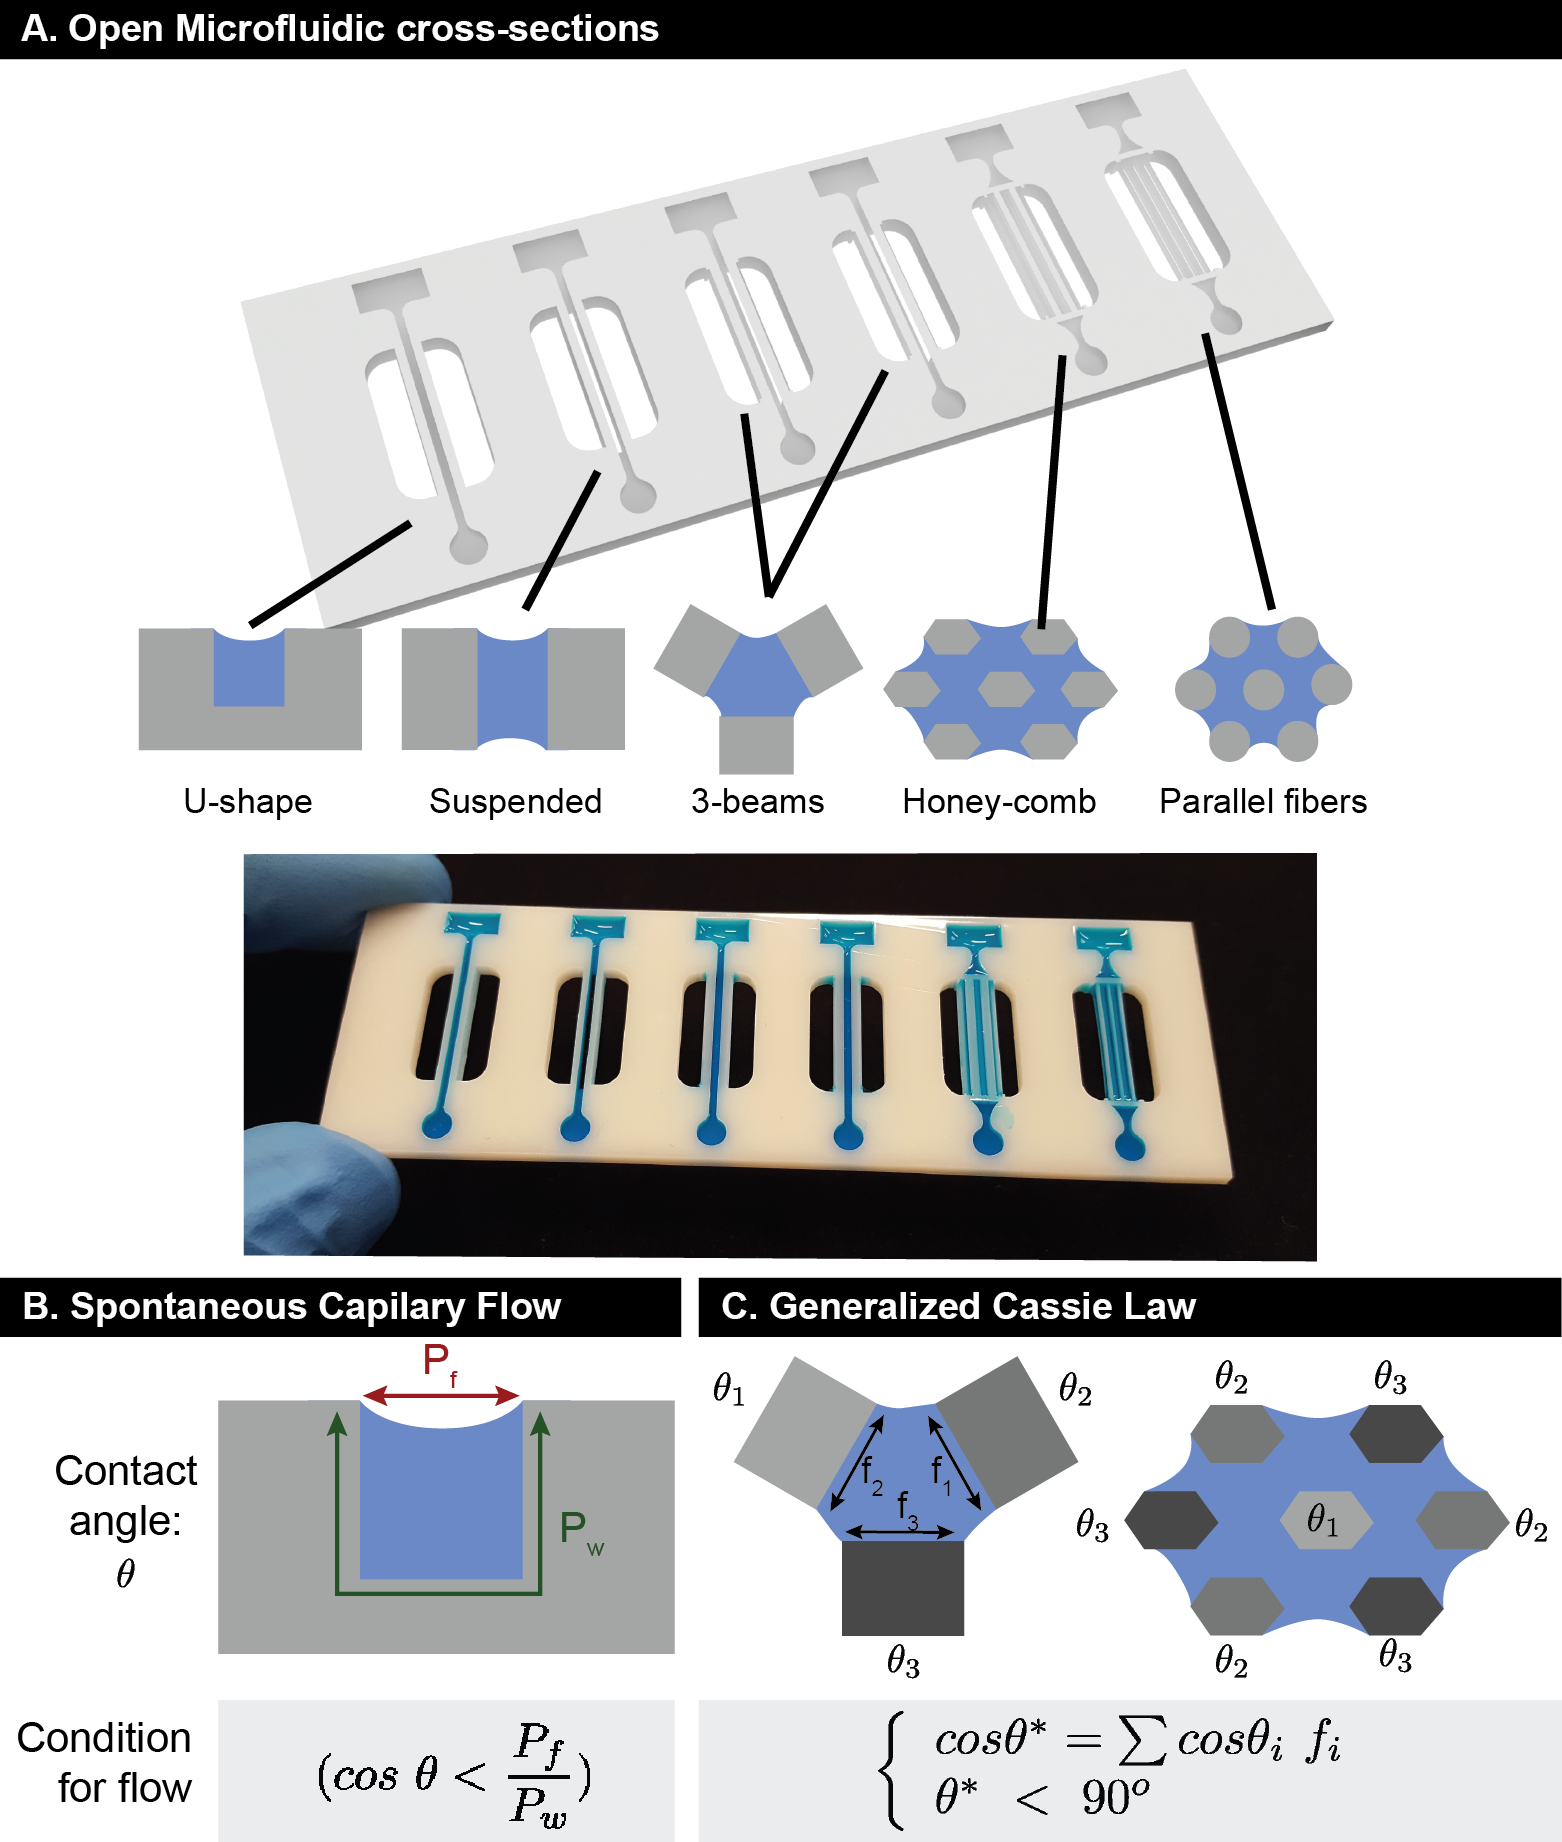
\includegraphics[width=5.0 in]{/OpenFig1.png}
\caption[\textbf{Open microfluidic concepts and generalization of capillary principles}]{\textbf{Open microfluidic concepts and generalization of capillary principles}. (A) 3D printed plate with different cross-sections of open microfluidic channels, including a rectangular groove, a suspended fluid, and suspended beams. (B) Condition for flow in a simple open microfluidic channel in which all the solid faces of the material contacting the fluid have the same contact angle (\texttheta). The perimeter of the cross-section of the channel forming the air-liquid interface is noted P$_f$ and the perimeter of the cross-section of the channel forming the solid-liquid interface is noted P$_w$ \cite{Berthier2012SuspendedStudies}. (C) Generalization of the Cassie law stating the condition for flow in an open microchannel of any cross-section including materials of different compositions or contact angles \cite{Berthier2014AMicrochannels}.}
\label{figure:Fig1}
\end{figure}


\subsection{Open microfluidic enables flow in 3 dimensional systems}
Microfluidic fabrication is a notoriously complex process that has been the subject of intense research \cite{Zhao2015, Becker2002, Becker2000a}. Traditionally microfluidic systems have been designed on planar surfaces such as glass, silicon, or plastic sheets as manufacturing and bonding processes are typically bound to 2D surfaces. Three-dimensionality can be obtained using 3D printing techniques where the channels are printed in bulk UV curable material \cite{Au20163D-PrintedMicrofluidics}, however intricate strategies must be developed in order to remove the uncured polymer from the channels. Further, closed system microfluidics suffers from important barriers of reliability (due to the potential for air bubbles blocking the channels) and usability (due to the need to seal the channel). The open nature of the channels also allows for robust and homogeneous treatment of the surfaces, such as plasma treatment, chemical vapor deposition, or spray coating \cite{Casavant2013, Piraino2012}.


Open microfluidics removes the requirement for bonding. Thus, open channels can be created on non-planar and 3-dimensional surfaces in which the fluid starts from a location and can follow a channel imprinted along multiple intersecting planes (Figure \ref{figure:Fig2}A,B). Using SLA printing we demonstrate that open microfluidic flows can occur in channels travelling through 2 intersecting planes at different angles (Figure \ref{figure:Fig2}A) as well as in vertical and even upside-down configurations (Figure \ref{figure:Fig2}B). Further, open microfluidics truly allows flows in non-planar configurations such as curved faces that can only be realized in 3D printing or high-end micromilling (Figure \ref{figure:Fig2}C). Another important design feature of open microfluidics consists in the potential of creating a sideways filaments (Concus-Finn filament) at inflexion points in the path of the (Figure \ref{figure:Fig2}D). A simple solution is adding a fillet between the 2 planes with a radius inversely proportional to the angle between the 2 planes.

\begin{figure}[h!] %DONE
\centering
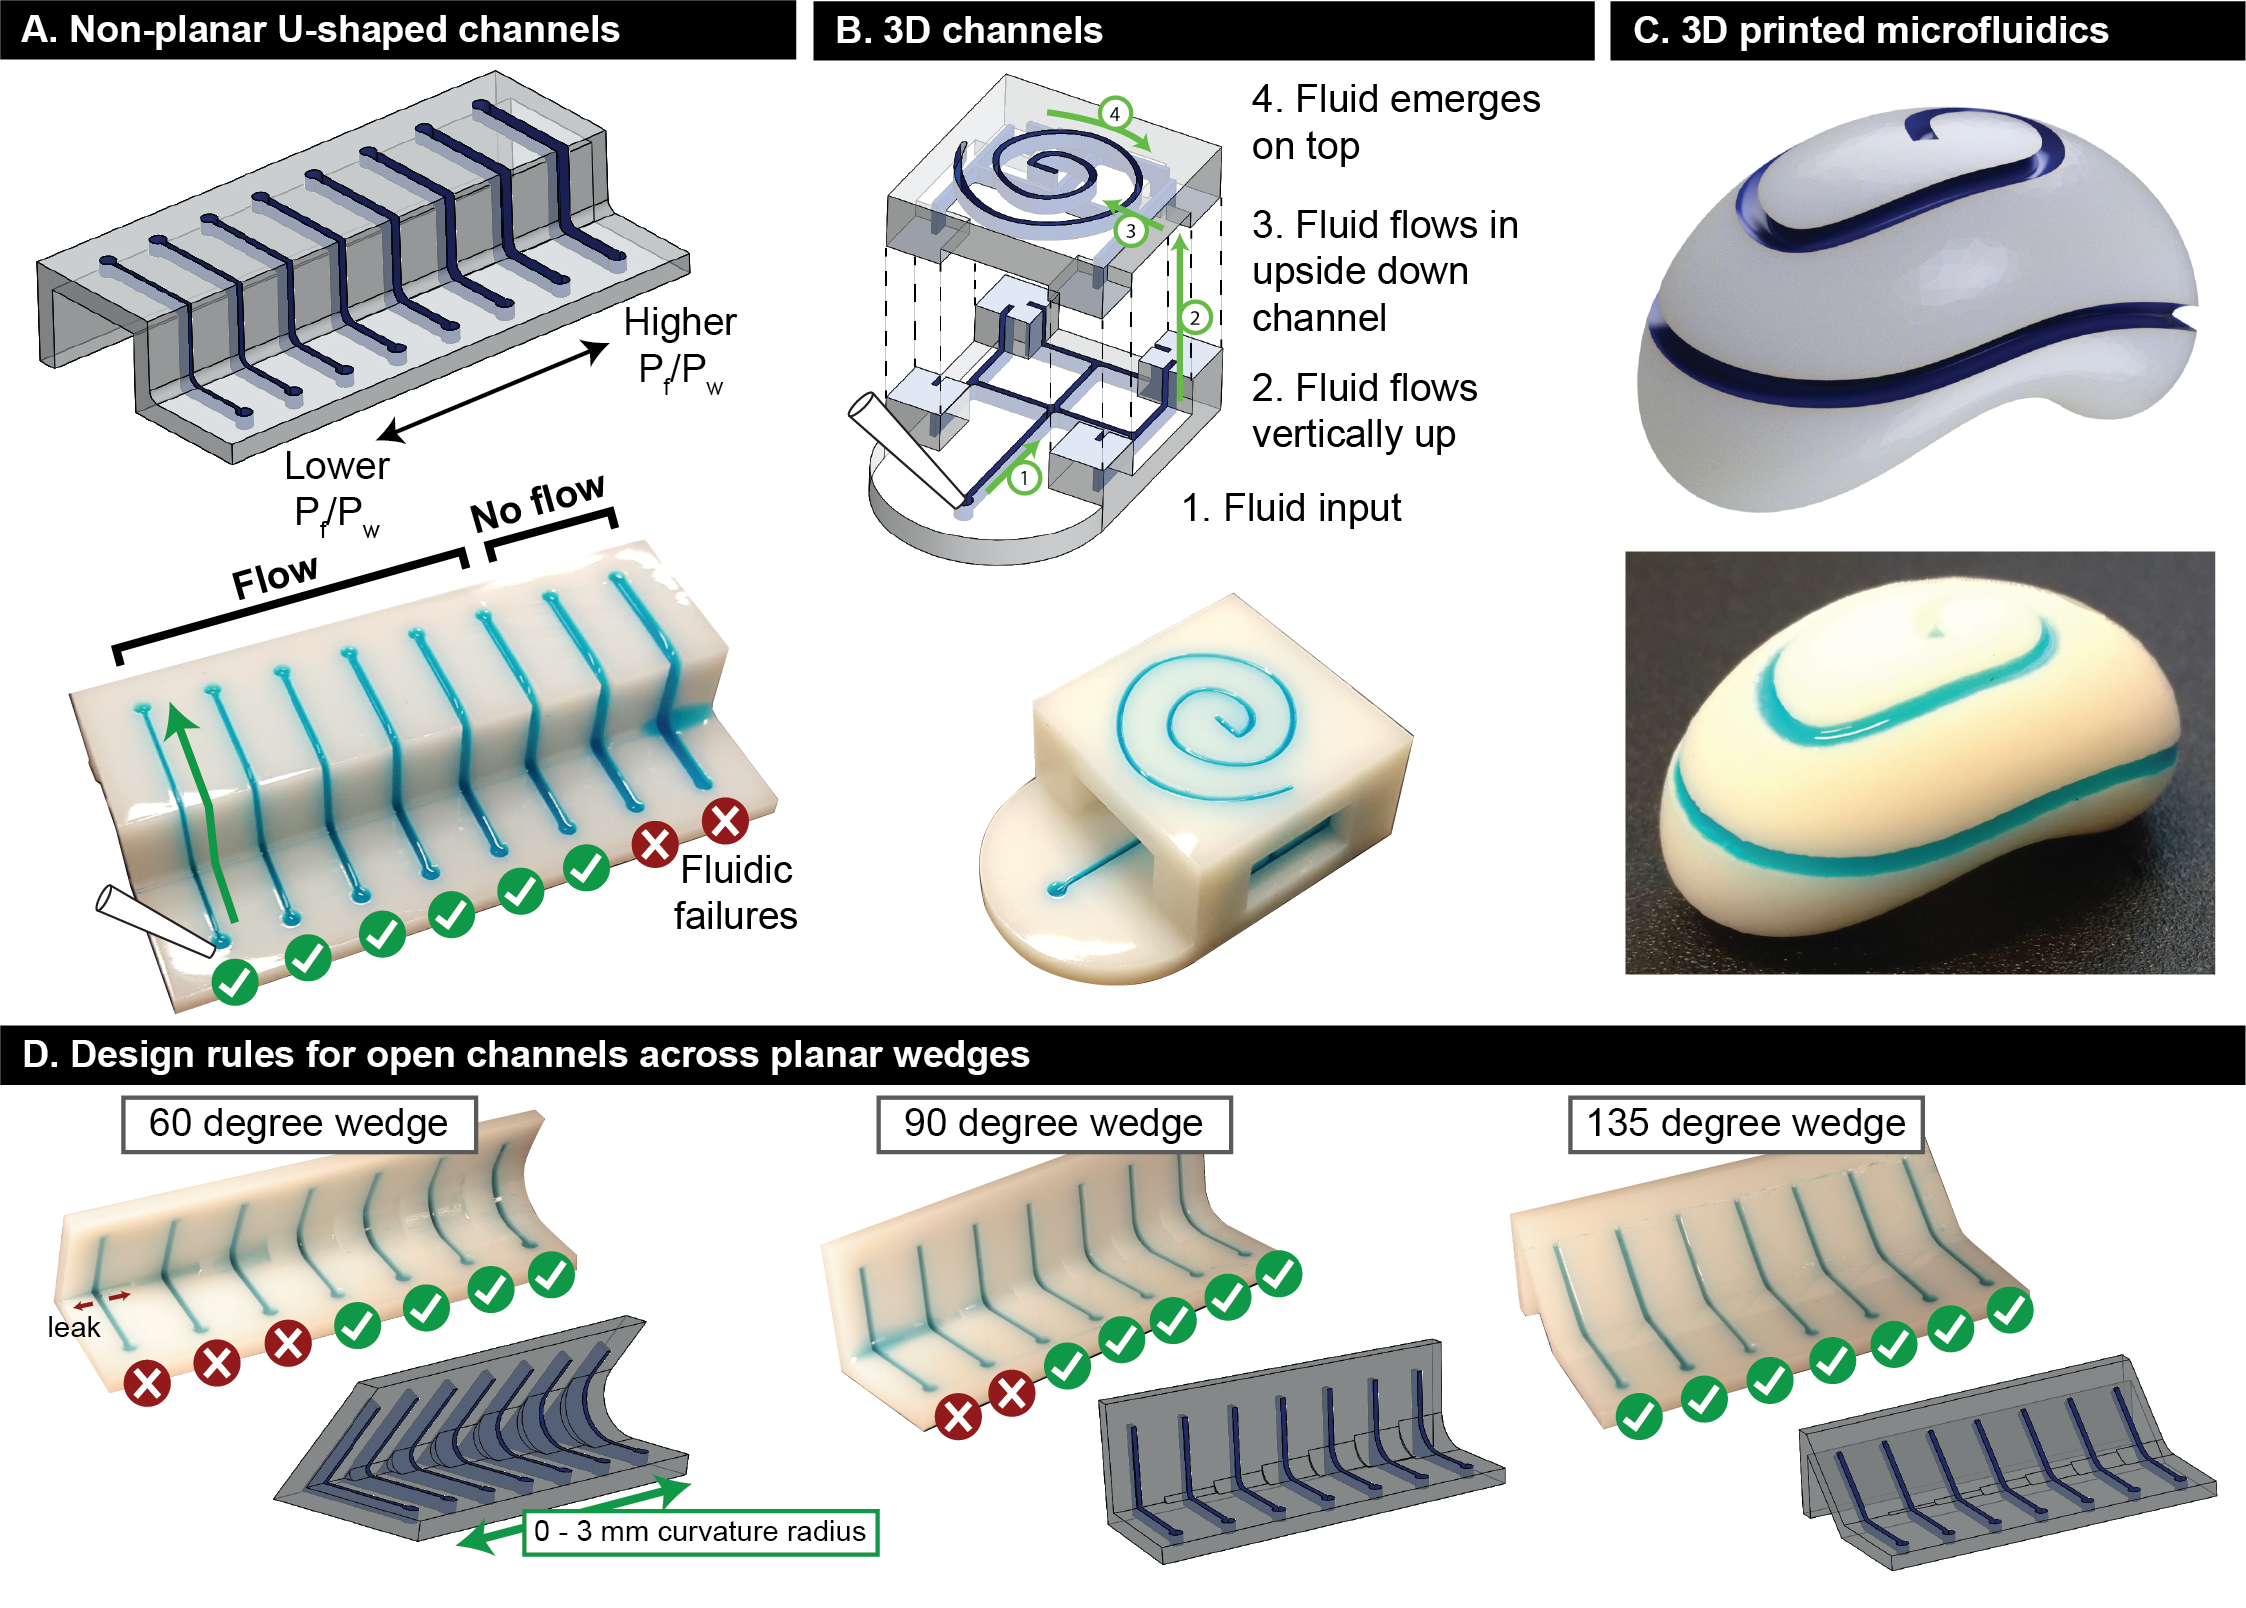
\includegraphics[width=5.0in]{/OpenFig2.png}
\caption[\textbf{Examples of open microfluidic channels}]{\textbf{Examples of open microfluidic channels}. (A) Example of a rectangular cross-section channel flowing up a stepwise channel. A range of width of channels represent different conditions of the SCF equation. When the aspect ratio of the channel passes a certain threshold value, flow is prevented. (B) Example of flow in a complex multifaceted surface designed by SLA printing in which the fluidic path diverges from the horizontal plane. (C) An open microfluidic channel carved into a miniature representation of "The Bean" sculpture displayed at the millennium park in Chicago, Illinois. (D) Design considerations for channels running across wedges between 2 planes.}
\label{figure:Fig2}
\end{figure}

Open microfluidics do not suffer from critical failure modes due to trapped air-bubbles. The inherent nature of open microfluidics allows air to escape at any point along the length of the channel. Thus, any air gap created by timing errors, or pipetting errors, are resorbed or outgassed within the channels. Gravity-effects, however, must be taken into consideration when working in 3D geometries that are made possible by open microfluidics. We analytically derived a generalized calculation for the maximum vertical height that a fluid inputted in an open microchannel may travel (Equation \ref{equation:Eq1}) and can be thought of as the equivalent of the capillary strength calculated in closed capillary microfluidic systems. 

\begin{equation}
    \Delta h= \frac{\sum f_{i}\gamma cos(\theta )}{\rho gA}
    \label{equation:Eq1}
\end{equation}

\subsection{Open microfluidic breadboard system using Lego\textregistered\, blocks}
A breadboard approach to development of microfluidic platforms has long been an aspiration of microfluidic designers and engineers; allowing to rapidly test concepts and cut down prototyping and manufacturing time. Several reconfigurable or modular microfluidics approaches have been proposed \cite{Bhargava2014, Chen2011, Frey2014,Shaikh2005}, however, they suffer from manufacturing complexity and sealing and reliability challenges. One of the requirement for a successful breadboard technology is that each unit is cost effective and allow ubiquitous reconfiguration. Using open microfluidics we developed a system that is inspired by the popular Lego\textregistered \, blocks. In particular the approach allows simple injection molding fabrication and assembly in many different configurations.

The prototyping platform consists of individual blocks with open channels that can be placed on any face of the block. Fluidic components of individual blocks interface with each other with a connector that prevents flow while blocks are separated. The connection consists of a vertical semi-circular open channel that terminates near the bottom of a block (Figure \ref{figure:Fig3}A). When filled the pressure is low enough such that the fluid at the end of the channel pins and is held by surface tension. The receptor on the next block in the interface is a tapered pin connected to the open fluidics on its channel. When interfaced, the pin on the lower block breaks the surface tension of the droplet on the upper block and allows flow between blocks. The blocks themselves can be assembled with peg attachment system and can be interfaced with Lego\textregistered \, blocks for use as scaffolding (Figure \ref{figure:Fig3}B). The interface at both the fluidic and block level is designed so that individual blocks such as sources and receptacles are easily interchangeable and replaceable and will not result in spilling of fluid allowing for prototyping multi-step or time-based circuits. With this template we can incorporate microfluidic operation onto the blocks, each block has a commonly used microfluidic function like valving, combining fluids, and mixing (Figure \ref{figure:Fig3}C). Functional blocks can be assembled into open microfluidic circuits that are not only modular, but reconfigurable during operation. Figure \ref{figure:Fig3}D demonstrates a completed open microfluidic circuit and its operation. Fluids can be preloaded in blocks, like reservoir blocks and valved blocks before being initiated. Since it is open, the circuit can be manipulated with a pipette at any place along the fluid path and at any time. Wash cycles in this circuit are achieved by adding preloaded reservoir blocks.


\begin{figure}[h!] %DONE
\centering
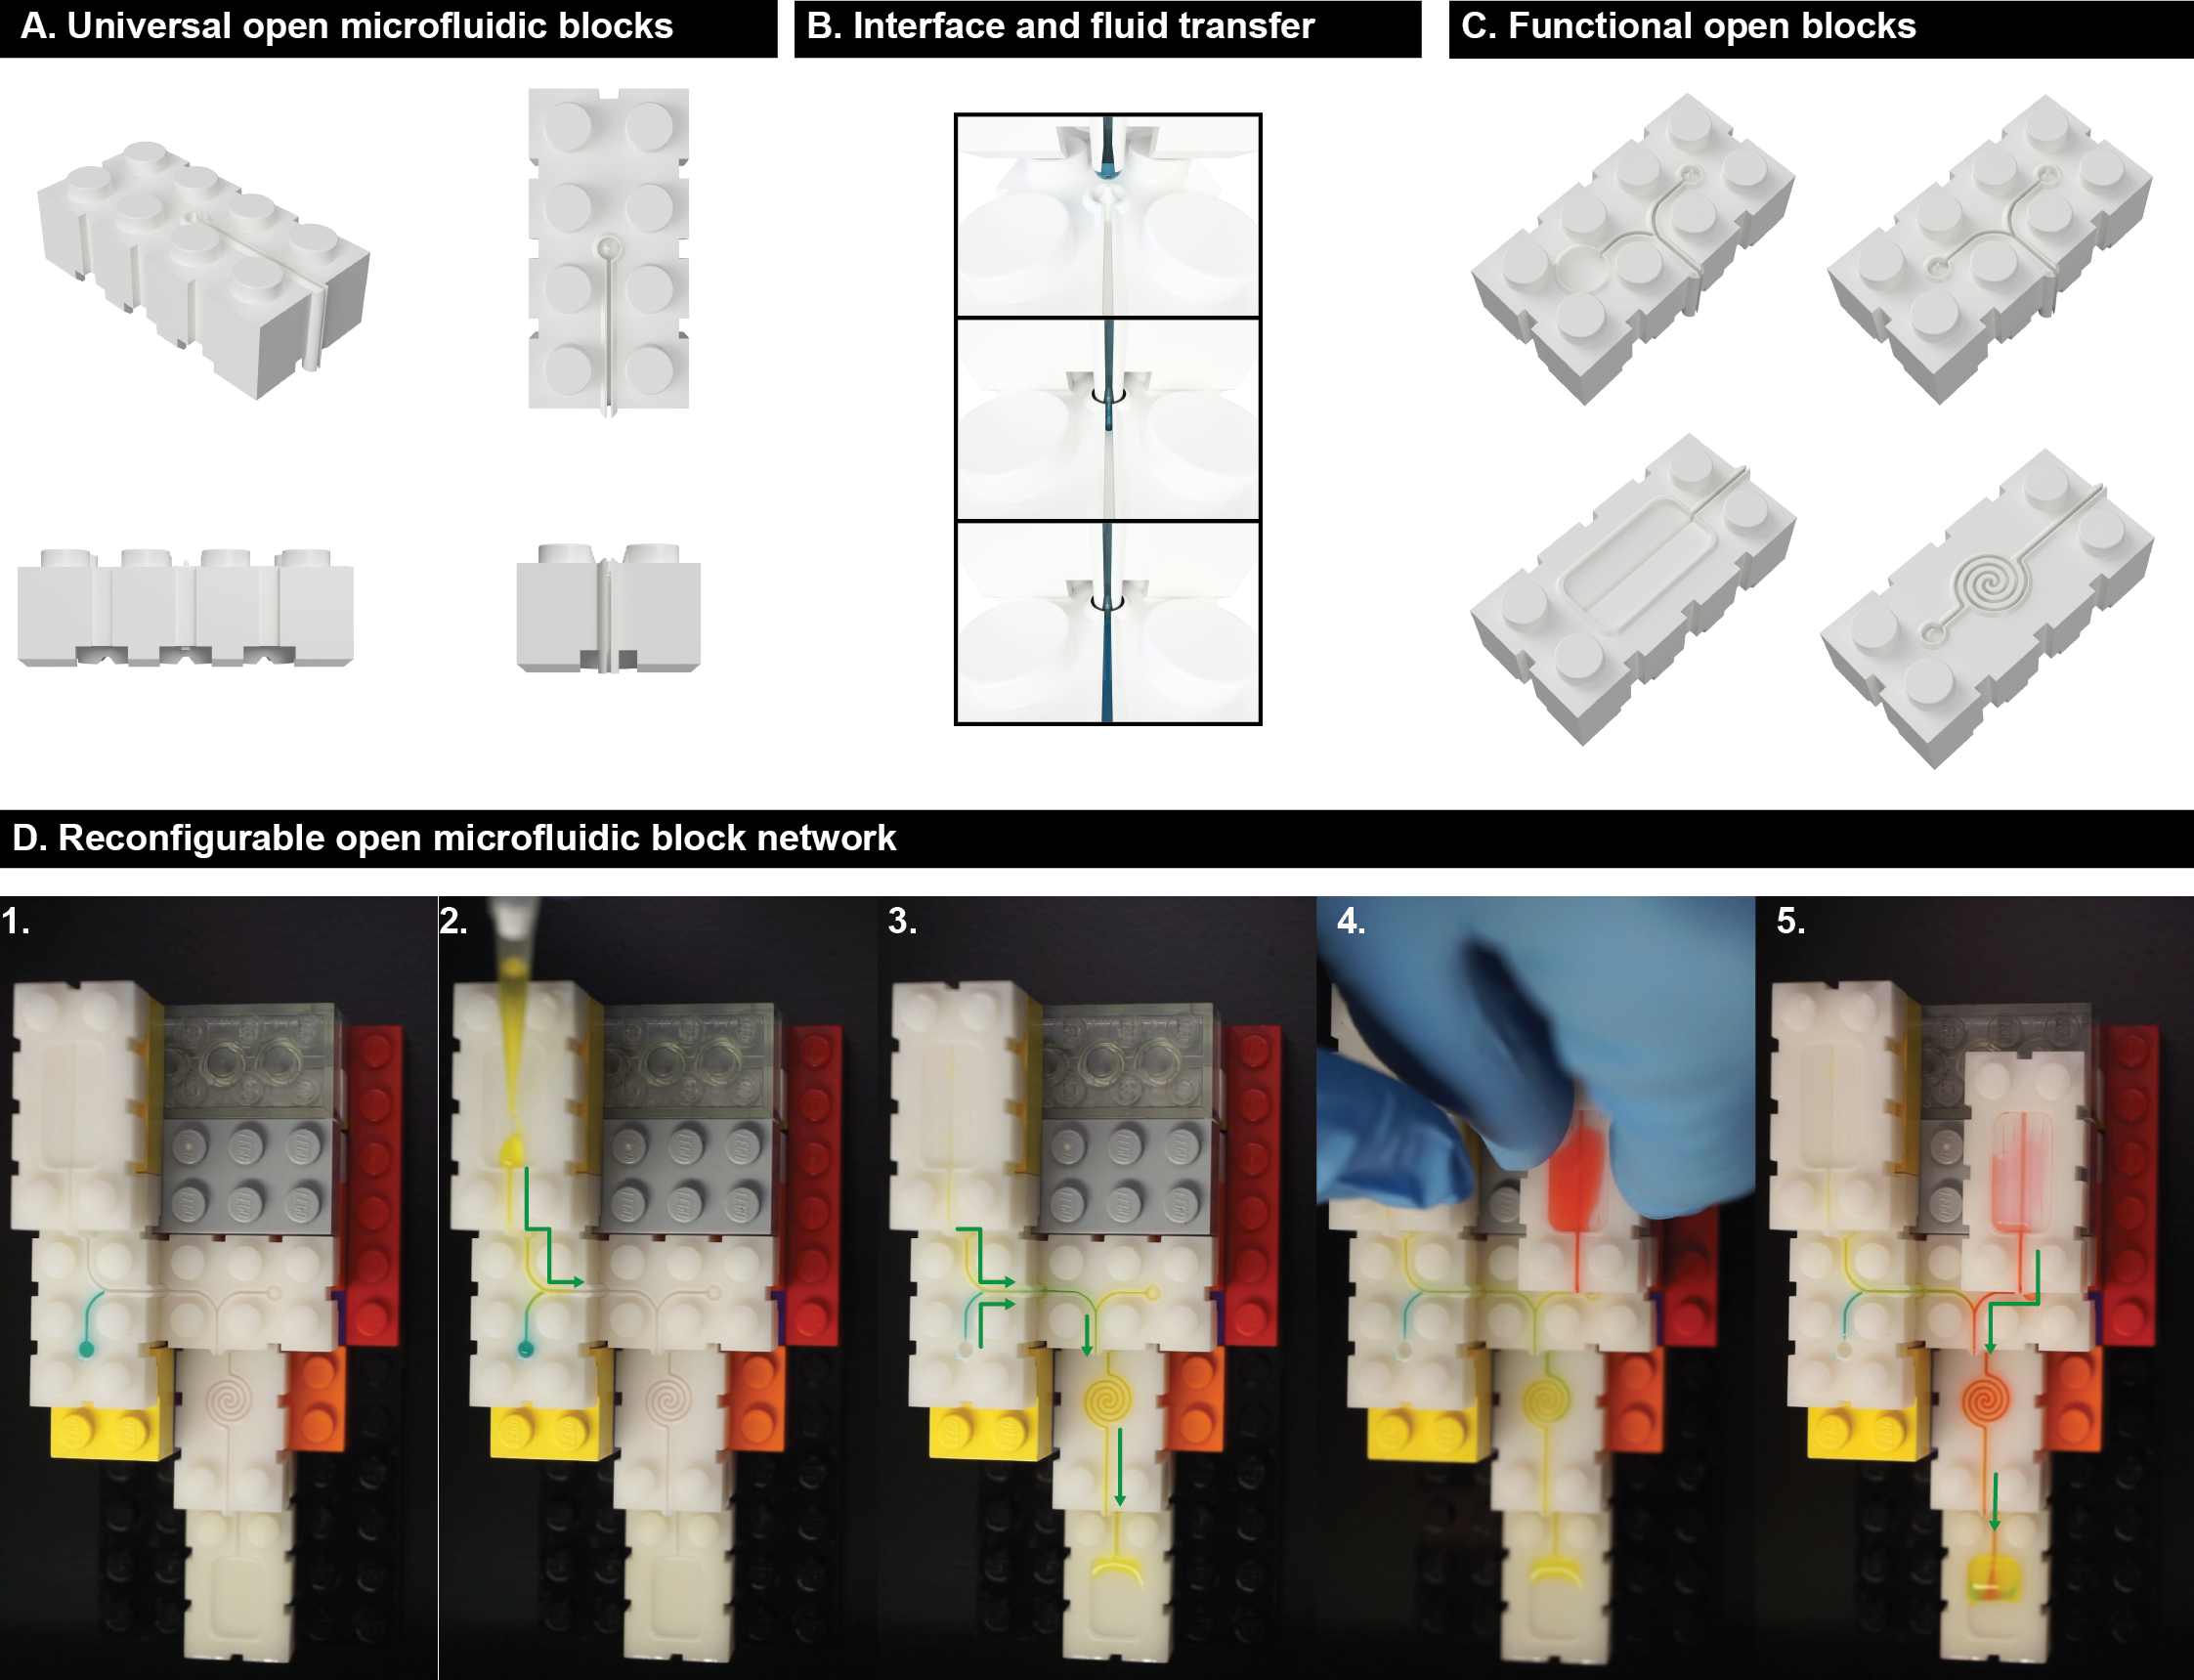
\includegraphics[width=5.4in]{/OpenFig3.png}
\caption[\textbf{A reconfigurable open microfluidic platform}]{\textbf{A reconfigurable open microfluidic platform}. (A) Standard reconfigurable block with straight channel. (B) Blocks are interfaced with one another by direct connection and can be configured in multiple orientations. (C) Connector between contains fluid to individual blocks until connection in made. Pin in receiver block breaks the pinned fluid in the source block and enables fluid flow. (D) Interfacing blocks with functional channeled designed into the surface. (E) Time-lapse images of microfluidic circuit created by combining a set of functional reconfigurable blocks.}
\label{figure:Fig3}
\end{figure}

\subsection{Reconfigurable open microfluidic systems}
Open microfluidics allows the design of moving microfluidic networks. We have shown that open microfluidics allows the design of reconfigurable networks during the operation of the fluidic flows, as illustrated by the Lego block networks in which blocks can be added at any point of the operation of the system (Figure \ref{figure:Fig4}4). We expanded the concept by developing microfluidic systems that can be operated while in constant movement, such as parts rotating relative to each other during the microfluidic flow. Moving channels can be interesting to develop applications in which constant-flow microfluidic flows are separated into discrete fluid aliquots such as used in digital microfluidic applications. 
We demonstrate a microfluidic system that transforms a constant fluid flow into discrete fluidically independent aliquots. We developed a ferris-wheel type device that is able to rotate relative to a feeder channel. The important criteria to design the rotating device are (1) designing a system for fluidic exchange between the 2 parts (i.e. in which fluid can flow from one channel to the other) and (2) designing a connection that can come in and out of fluidic connection in a constant movement and be repeated. Here, to create the feeder channel, we deigned an open channel with no ceiling and which contains slots in the front and back allowing the wheel to enter the feeder channel, move through it, and exit at the end (Figure \ref{figure:Fig4}A). By making the feeder channel circular around a central axis, the wheel is able to rotate around the axis and each branch of the wheel can in turn connect with the feeder channel, fill with fluid, and disconnect. Using open microfluidics, we were able to bring an input channel to the feeder channel along the sides of the base structure. In this example the input channel may be connected to a constant fluid flow or connected to any reservoir of fluid, and the Ferris wheel will aspirate constant volumes of fluid (as defined by the geometry of the channel) from the input flow. 
Pursuing on systems that enable the conversion of constant fluid flows into digital microfluidic systems, we demonstrate the potential for open microfluidics to acquire arrayed aliquots of fluid. In particular, we show that using open microfluidic systems fluid can be exchanged between two microfluidic parts in a way that enables the full enclosure of the arrayed fluids. To achieve this, we designed a microfluidic channel that presents an array of raised cylindrical sections. A second microfluidic part that presents an array of wells with a capillary transfer geometry connects to the initial plate, transfers the fluid into the wells, and importantly keep the surface of the fluid below the surface of the plastic. This approach allows the arrayed microwells to be enclosed using tape or a lid in order to perform a desired reaction such as a PCR reaction while preventing evaporation. 

\begin{figure}[h!] %DONE
\centering
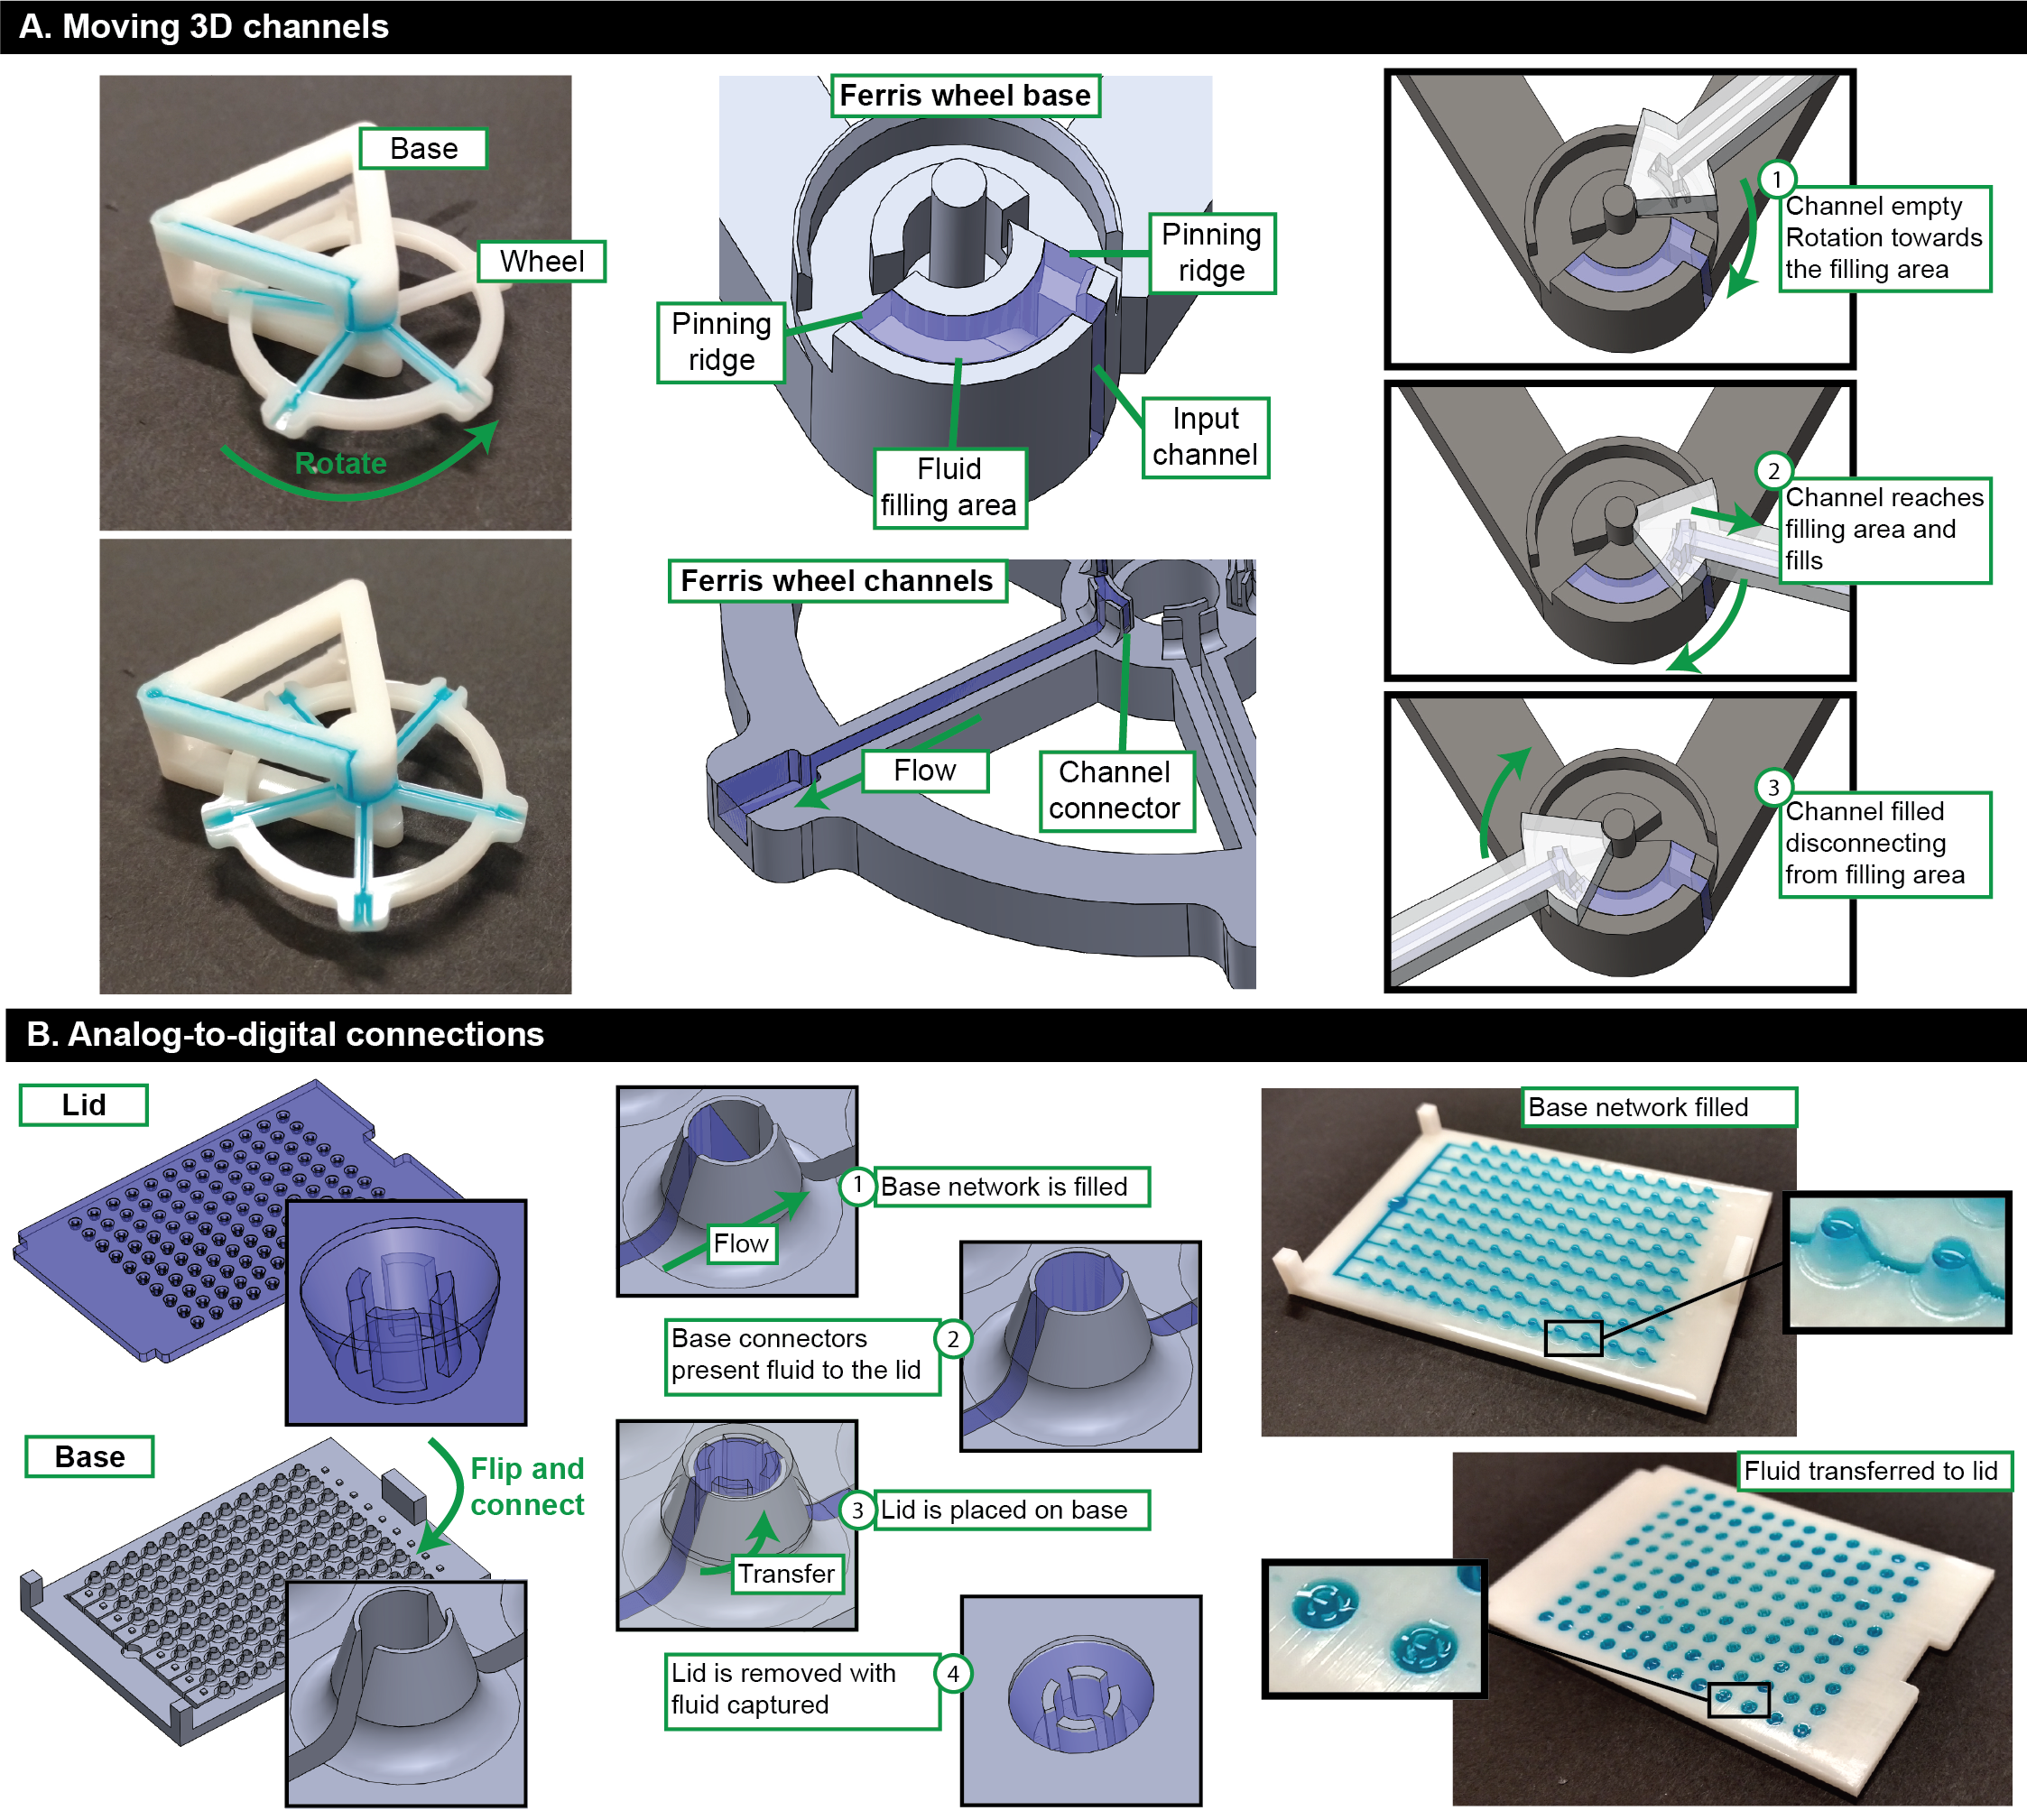
\includegraphics[width=5.2 in]{/OpenFig4.png}
\caption[\textbf{A reconfigurable open microfluidic platform}]{\textbf{A reconfigurable open microfluidic platform}. (A) Standard reconfigurable block with straight channel. (B) Blocks are interfaced with one another by direct connection and can be configured in multiple orientations. (C) Connector between contains fluid to individual blocks until connection in made. Pin in receiver block breaks the pinned fluid in the source block and enables fluid flow. (D) Interfacing blocks with functional channeled designed into the surface. (E) Time-lapse images of microfluidic circuit created by combining a set of functional reconfigurable blocks.}
\label{figure:Fig4}
\end{figure}

\section{Conclusions}
Open microfluidics offers considerable benefits over traditional closed systems. It offers fluid manipulation that is precise and controllable but is accomplished passively, without the need for external pumps. Open microfluidic systems are simple to fabricate since bonding is not required, and amenable to 3D printing allowing rapid dissemination of designs. Fluid flow is spontaneous in open microfluidics and fluid is open channels is accessible throughout the entire channel through pipette or build in sampling. We have demonstrated several capabilities of open microfluidic systems that can be built on to create a range of devices with applications in everything from chemistry to education. 

\section{Design notes for open microfluidic devices}
While open microfluidic systems avoid many common causes of device failure that are experienced by traditional closed systems such as bubbles, there are several scenarios in which device material and geometry will lead to failure including leakage and loss of spontaneous capillary flow.

Sharp corners in both open and closed microfludic channels are problematic and lead to device failure. In closed systems it has been observed that corners will lead to failure through the formation of air bubbles \cite{Liu2015}. Sharp corners in the horizontal-plane of both open and closed capillary flow-driven channels have the effect of pinning fluid which can slow or even stop flow in the channel. In open channels this can result in leakage upstream of the corner as the pressure required to break the pinning can be greater than the pressure keeping fluid contained within the channel. To failures at channel corners, sharp corners should be avoided all together. Filleting channel corners prevents unintended fluid pinning and will reduce the chances of failure in the device. Sharp corners in the vertical plane, such as those used in \ref{figure:Fig2} A, B, and D can fail not only due to pressure of gravity but also by satisfying the conditions required to form a Concus-Finn filament described in equation \ref{equation:Eq2} in which \texttheta is the contact angle between the fluid and the channel and a is angle of the corner.

\begin{equation}
    \theta < \frac{\pi }{2}-\frac{a}{2}
    \label{equation:Eq2}
\end{equation}

Smaller corner angles have a higher potential to result in the formation of Concus-Finn filaments \cite{Berthier2015a} resulting in devices leakage and failure. As discussed in section 4.3.2, failures can be reduced in open channel corners by both increasing ratio of P$_w$ to P$_f$ and by including a radius of curvature at the corner to reduce corner effects of spilling. 

To engineer channels that will be more resistant leakage from the channel tops, channel edges can be designed with geometries of 90 \textdegree \, or greater. This is achieved by raising the edges of a channel above the surface of the device and connecting them back to the device outwards of the channels to create triangular cross-section on each edge of the channel. This approach was used to keep fluid within the reconfigurable open microfludic blocks. Selective hydrophobic patterning of areas where fluid is undesired is another approach to keeping fluid within the channel and to prevent leaking.

Flow control in an open channel design can also be achieved by modifying the P$_w$ to P$_f$ ratio or perhaps more difficulty, changing the hydrophilicity of the channel material. The more amenable a channel is to SCF, the faster the flow rate can be achieved \cite{Berthier2016}. Changing these parameters over the length of a channel can result in variable flow, however, care must be taken to prevent pinning and complete flow stoppage.

The key to engineering successful open microfluidics is to design channels in such a way to ensure that SCF is encouraged throughout the length of the channel and to avoid unintentional fluid pinning. When fluid is stopped it can result in device leakage and failure as pressure builds upstream of the fluid stoppage. Simple design guidelines like avoiding sharp corners and geometrically enforcing large contact angles can greatly reduce the probability of device failure and increase the chances of building a robust and operational device. 